% =====================================================================
%  Figure captions for the ten validation panels of
%  "On the Necessary Substructures of Finite Contact Graphs".
%  Each panel is one row of four data-driven charts (>=1 in 3D), white
%  background, minimal in-figure text. All series are computed from
%  explicitly constructed finite contact graphs (a medium vertex adjacent
%  to every part; edge weights at or above a floor), the same instances on
%  which the validation suite ran 149{,}793 checks across 600 graphs with
%  zero failures. Measurement is realised as a reshuffling: a
%  weight-preserving relabelling of the non-medium vertices.
% =====================================================================

% ---------------------------------------------------------------------
%  PANEL 1 -- Floor from Infinitude (the derived floor)
% ---------------------------------------------------------------------
\begin{figure*}[!htbp]
    \centering
    
\includegraphics[width=\textwidth]{figures/panel_1.png}
    \caption{\textbf{Floor from Infinitude: every thing carries a strictly positive identification residual.}
    (\textbf{A})~Identification residual of a thing---the boundary cost of a proper part---on the linear $y$-axis ($0.52$ to $130$) versus the floor $\beta$ on the linear $x$-axis ($0.5$ to $2.0$), $13{,}472$ parts over $\sim\!250$ instances. The red line is the equality $y=\beta$; every measured point lies on or above it, the content of Theorem~\ref{thm:floor-infinitude}: the comparison identifying a thing against the rest never completes, so the residual is positive.
    (\textbf{B})~Distribution of the dimensionless ratio residual$/\beta$ on the linear $x$-axis ($1.02$ to $64.8$), counts on the linear $y$-axis, threshold $1$ marked (red). The histogram is supported entirely at and above $1$: no thing has sub-floor residual.
    (\textbf{C})~Per-instance minimum residual on the linear $y$-axis ($0.52$ to $30.8$) versus floor $\beta$ on the linear $x$-axis ($0.5$ to $2.0$), $250$ instances; all points lie on or above the equality line, so the derived floor is strictly positive on every instance (Corollary~\ref{cor:floor-derived}).
    (\textbf{D})~Three-dimensional surface of the per-instance minimum residual over vertex count ($4$ to $8$) and floor ($0.5$ to $2.0$), $250$ instances, viridis colourmap; strictly positive throughout. Viewing angle: elevation $22^{\circ}$, azimuth $-60^{\circ}$.}
    \label{fig:panel-ground}
\end{figure*}

% ---------------------------------------------------------------------
%  PANEL 2 -- T0 Floor Theorem
% ---------------------------------------------------------------------
\begin{figure*}[!htbp]
    \centering
    
\includegraphics[width=\textwidth]{figures/panel_2.png}
    \caption{\textbf{T0, the Floor Theorem: no separation is sharp.}
    (\textbf{A})~Cut weight of every realisable part on the linear $y$-axis ($0.53$ to $104$) versus the floor $\beta$ on the linear $x$-axis ($0.5$ to $2.0$), $13{,}304$ cuts. The red line is $y=\beta$; every point lies on or above it, confirming Theorem~\ref{thm:floor}, $\wt(\partial U)\ge\beta>0$.
    (\textbf{B})~Distribution of cut$/\beta$ on the linear $x$-axis ($1.01$ to $63.4$), counts on the linear $y$-axis, threshold $1$ marked (red); supported entirely above $1$, so across all parts of all instances no cut is sharp.
    (\textbf{C})~Per-instance minimum cut on the linear $y$-axis ($0.53$ to $33.5$) versus floor ($0.5$ to $2.0$), $250$ instances, above the equality line.
    (\textbf{D})~Three-dimensional surface of the per-instance minimum cut over edge count ($3$ to $27$) and floor ($0.5$ to $2.0$), $250$ instances, plasma colourmap; strictly positive everywhere. Viewing angle: elevation $20^{\circ}$, azimuth $-55^{\circ}$.}
    \label{fig:panel-T0}
\end{figure*}

% ---------------------------------------------------------------------
%  PANEL 3 -- T1 Individuation by negation
% ---------------------------------------------------------------------
\begin{figure*}[!htbp]
    \centering
    
\includegraphics[width=\textwidth]{figures/panel_3.png}
    \caption{\textbf{T1, individuation by negation: a part is fixed by its complement.}
    (\textbf{A})~Part size $|U|$ on the linear $y$-axis ($1$ to $5$)\,---\,plotted as complement size $|\complement U|$ on the linear $x$-axis ($1$ to $7$)\,---\,over $13{,}430$ sampled parts; every part is determined together with its negation-set.
    (\textbf{B})~Distribution of the involution error $\lvert U\,\triangle\,\complement\complement U\rvert$ on the linear $x$-axis, a single bar exactly at $0$ (red), counts on the linear $y$-axis: complementation is an exact involution (Lemma~\ref{lem:involution}), so a part is recovered uniquely from its negation-set.
    (\textbf{C})~Sum $|U|+|\complement U|$ on the linear $y$-axis ($4$ to $8$) versus the whole $|V|$ on the linear $x$-axis ($4$ to $8$); all points on the diagonal $y=x$ (red), so a part and its negation-set partition the whole exactly.
    (\textbf{D})~Three-dimensional scatter of $(|U|,|\complement U|,|V|)$ over $|U|\in[1,5]$, $|\complement U|\in[1,7]$, $|V|\in[4,8]$, cividis colourmap; all points lie on the plane $|U|+|\complement U|=|V|$. Viewing angle: elevation $24^{\circ}$, azimuth $-58^{\circ}$.}
    \label{fig:panel-T1}
\end{figure*}

% ---------------------------------------------------------------------
%  PANEL 4 -- T2/T3 residual: conserved region
% ---------------------------------------------------------------------
\begin{figure*}[!htbp]
    \centering
    
\includegraphics[width=\textwidth]{figures/panel_4.png}
    \caption{\textbf{T2/T3, the residual is a conserved region, never a point.}
    (\textbf{A})~Global minimum-cut residual on the linear $y$-axis ($0.53$ to $37.0$) versus floor $\beta$ on the linear $x$-axis ($0.5$ to $2.0$), $200$ instances, above the equality line (red): the residual is bounded below by the floor (Theorem~\ref{thm:residual-region}).
    (\textbf{B})~Residual after a reshuffling on the linear $y$-axis versus residual before on the linear $x$-axis (both $0.53$ to $37.0$), $200$ instances; every point on the diagonal $y=x$ (red) to machine precision: the residual is invariant under reshuffling (Theorem~\ref{thm:residual-invariant}).
    (\textbf{C})~Distribution of the size of the smaller side of the minimum cut on the linear $x$-axis ($1$ to $2$), counts on the linear $y$-axis, threshold $1.5$ marked (red); mass at size $\ge2$ shows the residual is realised by multi-vertex regions. The standalone two-cluster witness attains residual $=\beta=1$ with both sides of size $3$ ($\{0,1,2\}\mid\{3,4,5\}$): a region, never a point (Corollary~\ref{cor:point-forbidden}).
    (\textbf{D})~Three-dimensional surface of the residual over floor ($0.5$ to $2.0$) and minimum-cut side size ($1$ to $2$), $200$ instances, viridis colourmap. Viewing angle: elevation $22^{\circ}$, azimuth $-60^{\circ}$.}
    \label{fig:panel-T2T3}
\end{figure*}

% ---------------------------------------------------------------------
%  PANEL 5 -- T4 private invariant
% ---------------------------------------------------------------------
\begin{figure*}[!htbp]
    \centering
    
\includegraphics[width=\textwidth]{figures/panel_5.png}
    \caption{\textbf{T4, every part carries a positive private invariant.}
    (\textbf{A})~Private invariant---a part's boundary cost to the medium---on the linear $y$-axis ($0.51$ to $50.7$) versus floor $\beta$ on the linear $x$-axis ($0.5$ to $2.0$), $1{,}276$ parts; all points on or above $y=\beta$ (red), so the invariant is positive for every part (Theorem~\ref{thm:private}).
    (\textbf{B})~Private invariant on the linear $y$-axis ($0.51$ to $50.7$) versus part degree on the linear $x$-axis ($1$ to $7$); bounded below by the floor independently of degree.
    (\textbf{C})~Distribution of invariant$/\beta$ on the linear $x$-axis ($1.02$ to $34.1$), counts on the linear $y$-axis, threshold $1$ (red); supported entirely above $1$.
    (\textbf{D})~Three-dimensional surface of the per-instance minimum private invariant over vertex count ($4$ to $8$) and floor ($0.5$ to $2.0$), $250$ instances, magma colourmap; strictly positive. Viewing angle: elevation $22^{\circ}$, azimuth $-58^{\circ}$.}
    \label{fig:panel-T4}
\end{figure*}

% ---------------------------------------------------------------------
%  PANEL 6 -- T5 selection requires a gate
% ---------------------------------------------------------------------
\begin{figure*}[!htbp]
    \centering
    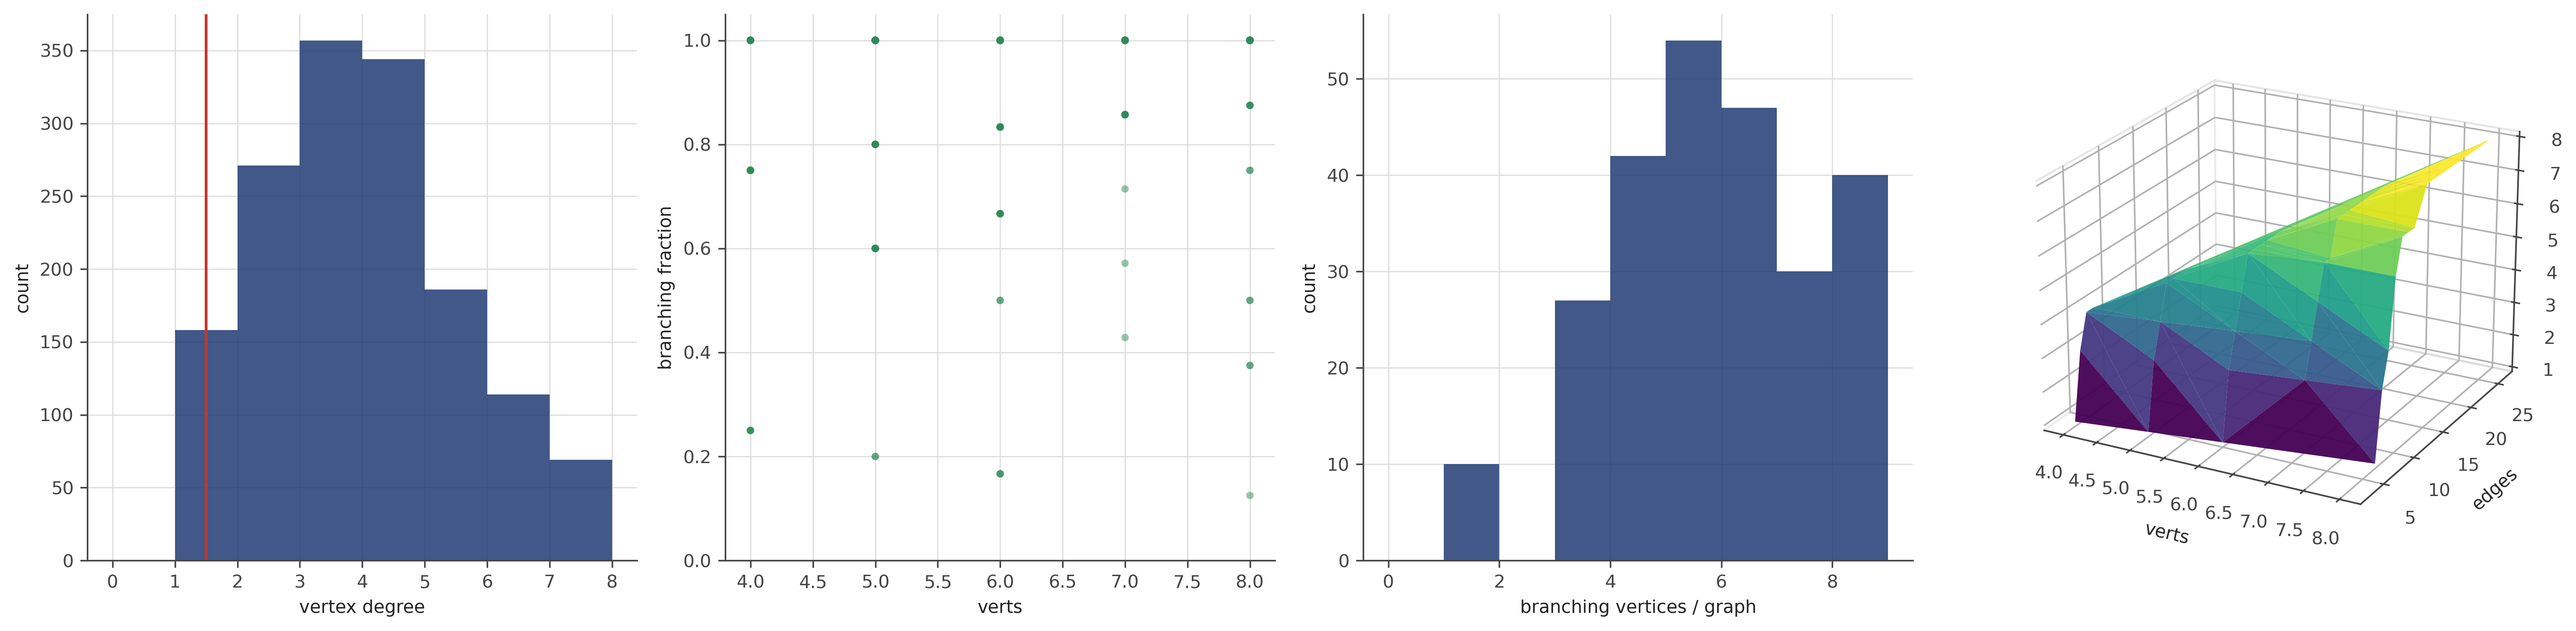
\includegraphics[width=\textwidth]{figures/panel_6.png}
    \caption{\textbf{T5, selection requires a gate: the graph underdetermines the next step.}
    (\textbf{A})~Distribution of vertex degree on the linear $x$-axis ($1$ to $7$), counts on the linear $y$-axis, $1{,}499$ vertices, threshold $1.5$ marked (red); the mass at degree $\ge2$ is the branching that leaves the next step undetermined by the graph alone (Lemma~\ref{lem:branching}).
    (\textbf{B})~Fraction of branching vertices per instance on the linear $y$-axis ($0.13$ to $1.0$) versus vertex count on the linear $x$-axis ($4$ to $8$), $250$ instances; near-total, so the graph fixes reachability but not order, and a gate is required (Theorem~\ref{thm:gate-necessary}).
    (\textbf{C})~Distribution of the number of branching vertices per instance on the linear $x$-axis ($1$ to $8$), counts on the linear $y$-axis.
    (\textbf{D})~Three-dimensional surface of branching-vertex count over vertex count ($4$ to $8$) and edge count ($3$ to $26$), $250$ instances, viridis colourmap. Viewing angle: elevation $22^{\circ}$, azimuth $-62^{\circ}$.}
    \label{fig:panel-T5}
\end{figure*}

% ---------------------------------------------------------------------
%  PANEL 7 -- T6 non-return
% ---------------------------------------------------------------------
\begin{figure*}[!htbp]
    \centering
    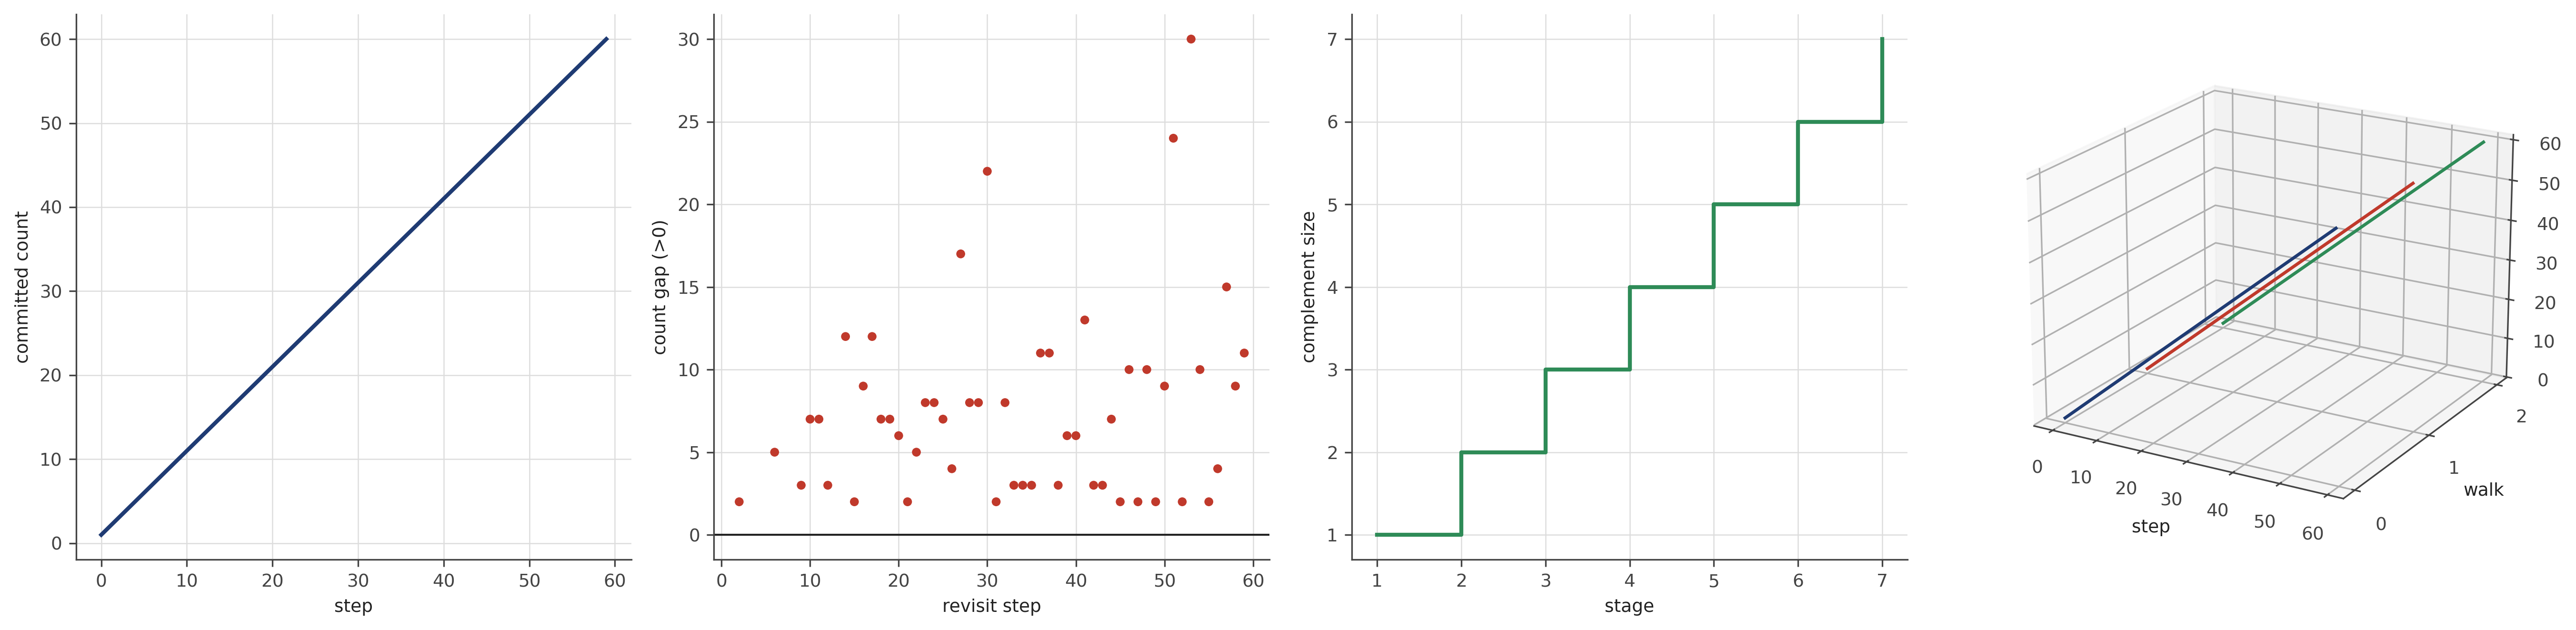
\includegraphics[width=\textwidth]{figures/panel_7.png}
    \caption{\textbf{T6, histories do not return: the committed count only grows.}
    (\textbf{A})~Committed count on the linear $y$-axis ($1$ to $60$) versus step on the linear $x$-axis ($0$ to $59$) along a gated walk; strictly increasing, so no state recurs (Theorem~\ref{thm:nonreturn}).
    (\textbf{B})~At every revisit of a vertex, the count gap to its previous visit on the linear $y$-axis ($2$ to $30$) versus the revisit step on the linear $x$-axis ($2$ to $59$), $52$ revisits; all gaps strictly positive (above the line at $0$): revisiting a vertex is never returning to a state.
    (\textbf{C})~Complement size of a fixed part on the linear $y$-axis ($1$ to $7$) versus the stage of a progressing whole on the linear $x$-axis ($1$ to $7$); monotone growth, so a thing is distinguishable from its own earlier stage (Theorem~\ref{thm:temporal-nonreturn}).
    (\textbf{D})~Three-dimensional overlay of three independent gated walks, committed count ($1$ to $60$) versus step ($0$ to $59$) at fixed walk-index, all strictly monotone. Viewing angle: elevation $20^{\circ}$, azimuth $-60^{\circ}$.}
    \label{fig:panel-T6}
\end{figure*}

% ---------------------------------------------------------------------
%  PANEL 8 -- T7 quotient inherits a floor
% ---------------------------------------------------------------------
\begin{figure*}[!htbp]
    \centering
    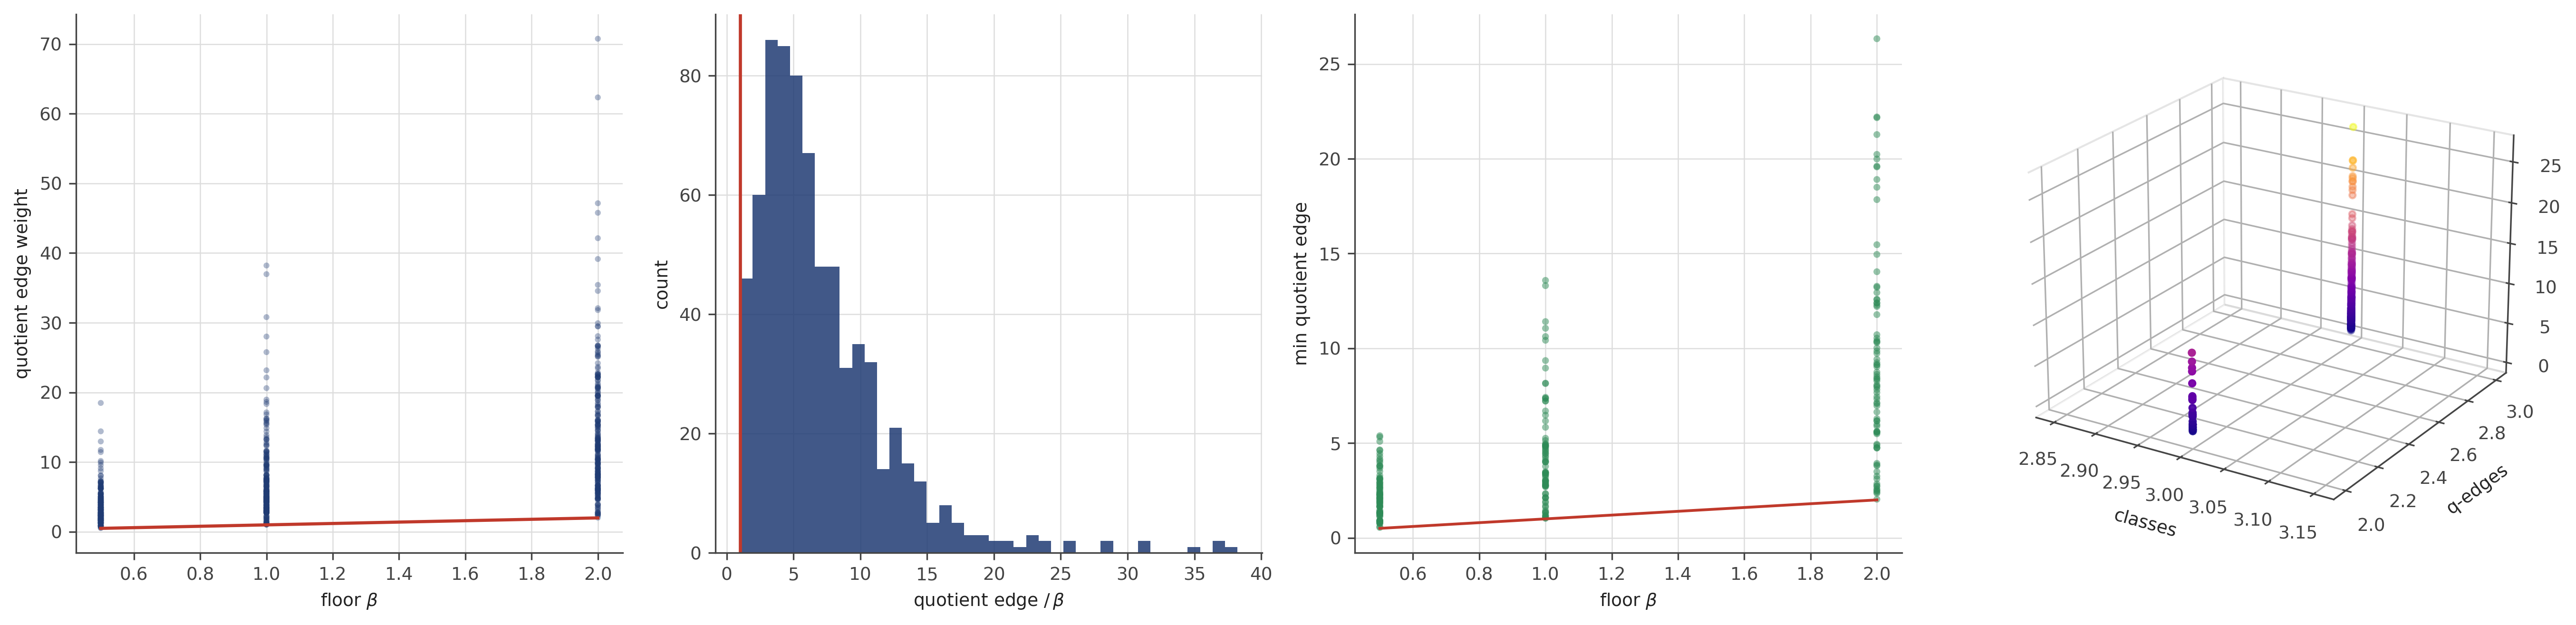
\includegraphics[width=\textwidth]{figures/panel_8.png}
    \caption{\textbf{T7, the quotient inherits a positive floor.}
    (\textbf{A})~Quotient edge weight---a class-to-class cut---on the linear $y$-axis ($0.55$ to $70.8$) versus floor $\beta$ on the linear $x$-axis ($0.5$ to $2.0$), $724$ quotient edges; all on or above $y=\beta$ (red), so the collective is again a contact graph (Lemma~\ref{lem:quotient-floor}).
    (\textbf{B})~Distribution of quotient-edge$/\beta$ on the linear $x$-axis ($1.02$ to $38.2$), counts on the linear $y$-axis, threshold $1$ (red); supported entirely above $1$.
    (\textbf{C})~Per-instance minimum quotient edge on the linear $y$-axis ($0.55$ to $26.3$) versus floor ($0.5$ to $2.0$), $250$ instances, above the equality line.
    (\textbf{D})~Three-dimensional surface of the minimum quotient edge over class count ($3$) and quotient-edge count ($2$ to $3$), $250$ instances, plasma colourmap. Viewing angle: elevation $22^{\circ}$, azimuth $-58^{\circ}$.}
    \label{fig:panel-T7}
\end{figure*}

% ---------------------------------------------------------------------
%  PANEL 9 -- T8 authored structures
% ---------------------------------------------------------------------
\begin{figure*}[!htbp]
    \centering
    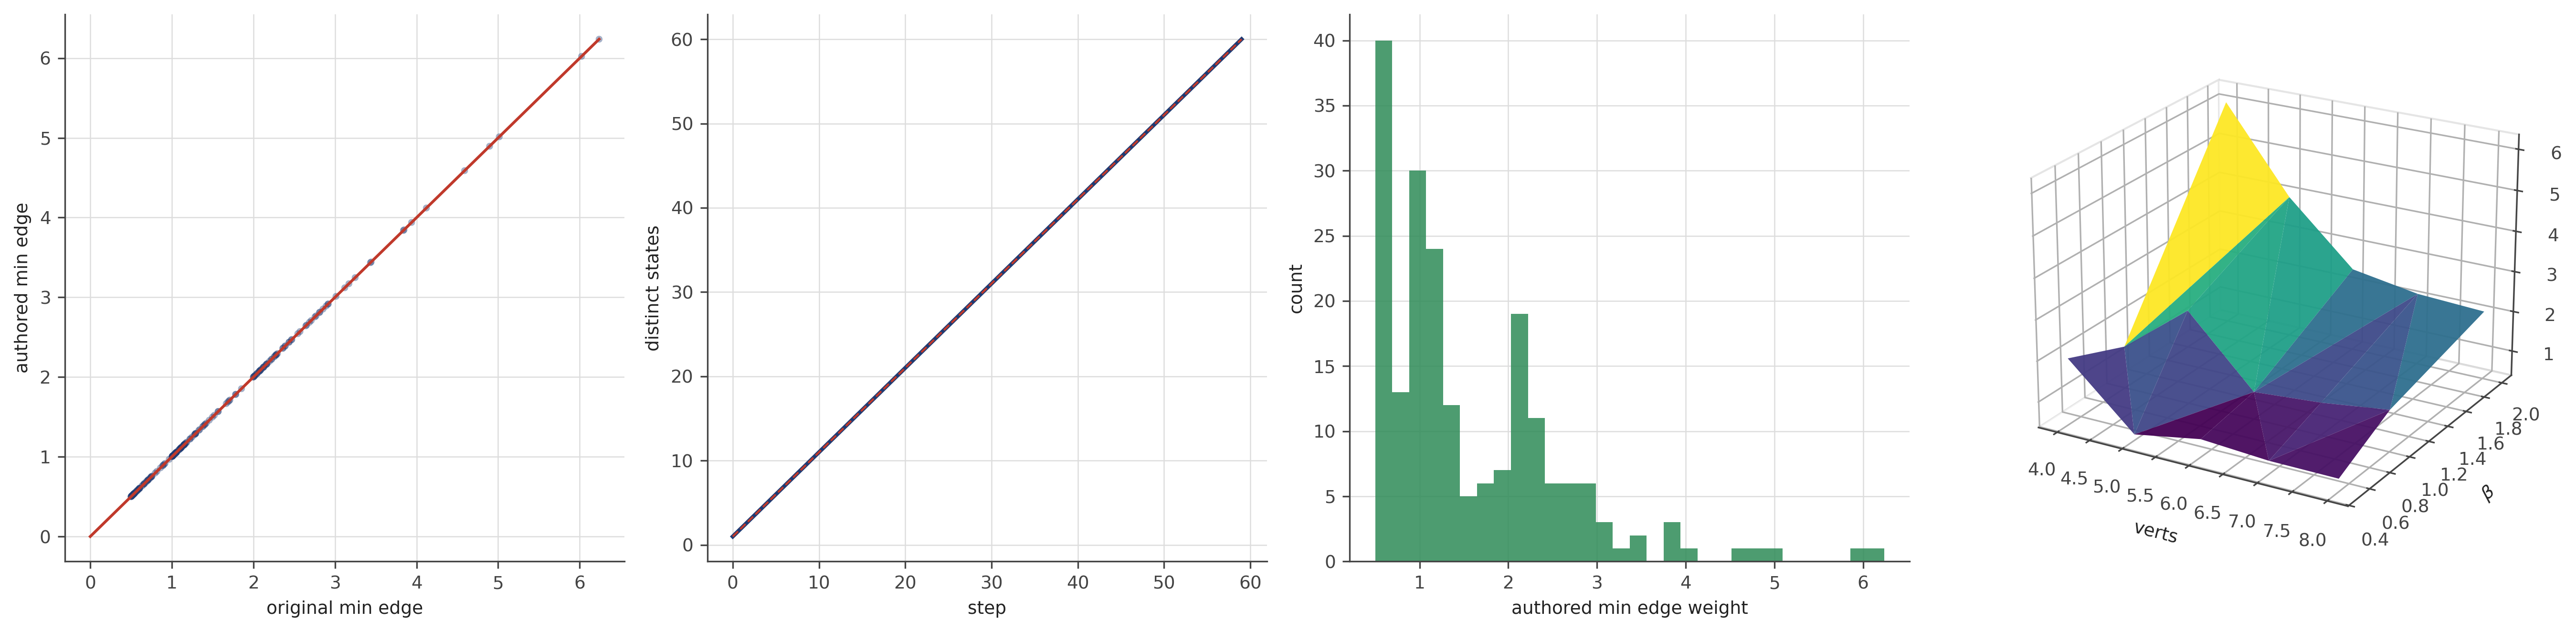
\includegraphics[width=\textwidth]{figures/panel_9.png}
    \caption{\textbf{T8, authored structures exist and are bounded.}
    (\textbf{A})~Minimum edge weight of an authored instance on the linear $y$-axis ($0.50$ to $6.24$) versus that of the original on the linear $x$-axis (same range), $200$ instances; every point on the diagonal $y=x$ (red): specify-then-instantiate preserves the floor (Theorem~\ref{thm:authored-exist}).
    (\textbf{B})~Distinct states of an authored structure's forward closure on the linear $y$-axis ($1$ to $60$) versus step on the linear $x$-axis ($0$ to $59$), tracking the unit-slope line (grey dashed): every state is new, so the forward closure is unbounded (open-endedness, Theorem~\ref{thm:open}).
    (\textbf{C})~Distribution of the authored minimum edge weight on the linear $x$-axis ($0.50$ to $6.24$), counts on the linear $y$-axis; bounded below by the floor---no sub-floor distinction is authorable (floor-limited authorship, Theorem~\ref{thm:floor-limited}).
    (\textbf{D})~Three-dimensional surface of the authored minimum edge over vertex count ($4$ to $8$) and floor ($0.5$ to $2.0$), $200$ instances, viridis colourmap; never sub-floor. Viewing angle: elevation $22^{\circ}$, azimuth $-60^{\circ}$.}
    \label{fig:panel-T8}
\end{figure*}

% ---------------------------------------------------------------------
%  PANEL 10 -- Measurement
% ---------------------------------------------------------------------
\begin{figure*}[!htbp]
    \centering
    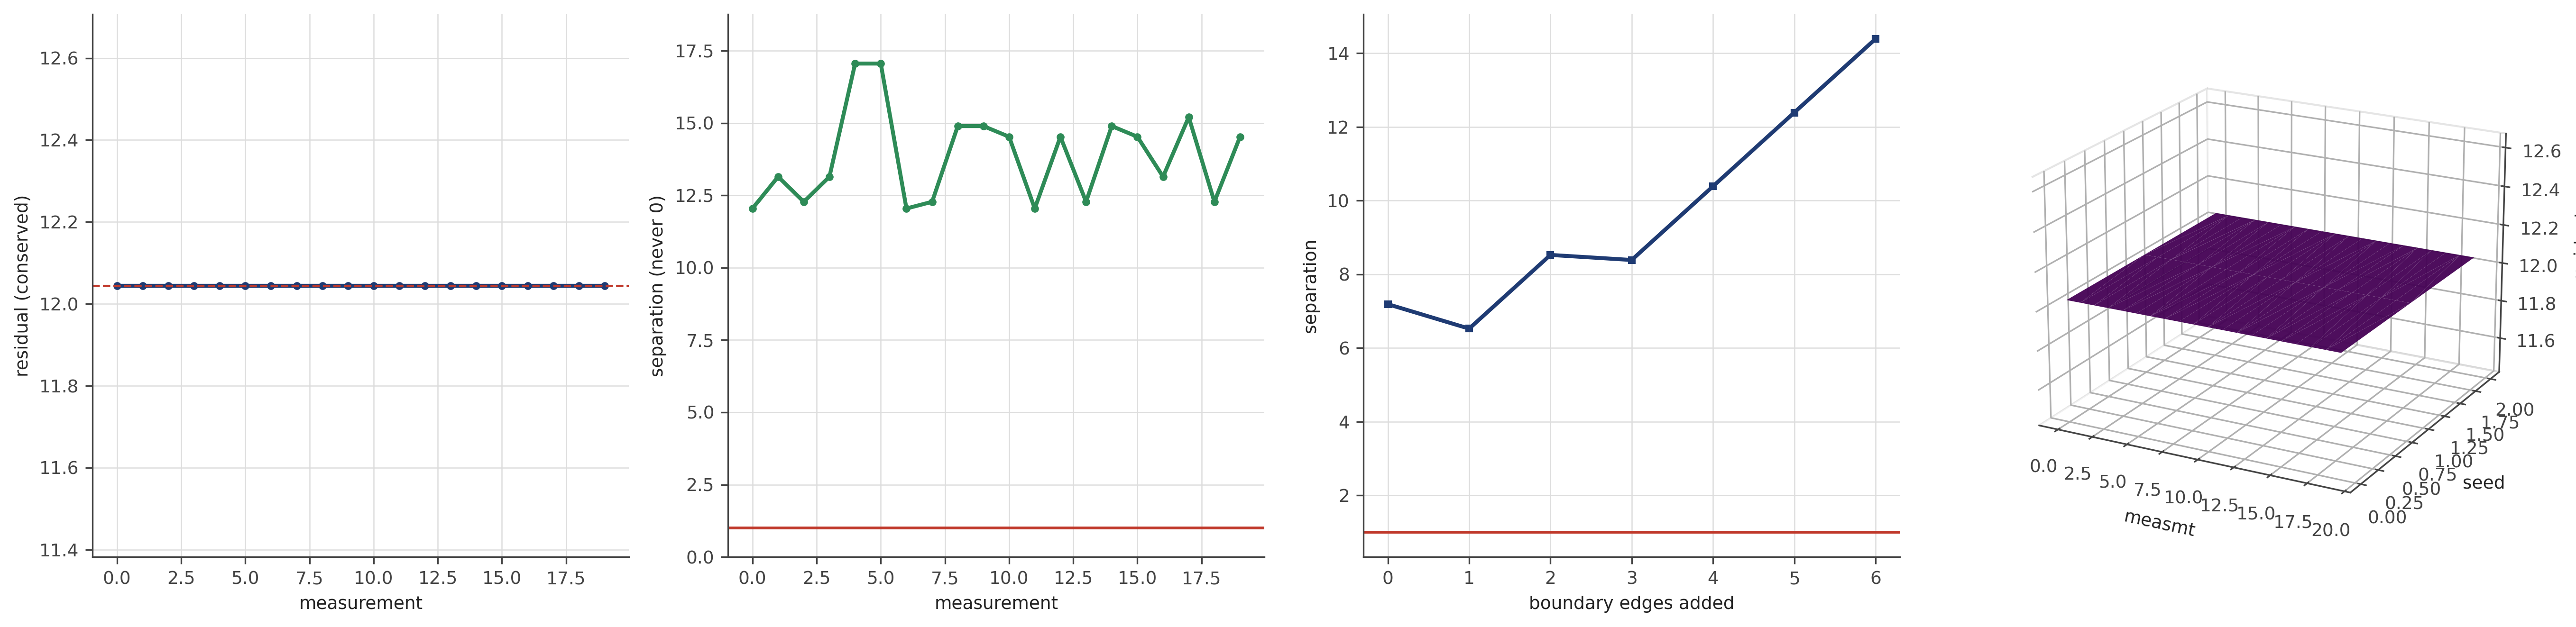
\includegraphics[width=\textwidth]{figures/panel_10.png}
    \caption{\textbf{Measurement: the invariant is conserved and identity is unreachable.}
    (\textbf{A})~Residual on the linear $y$-axis versus measurement index on the linear $x$-axis ($0$ to $19$) across $20$ successive reshufflings; a flat line at its initial value $12.045$ (red dashed): measurement conserves the invariant residual (Proposition~\ref{prop:measure-conserves}).
    (\textbf{B})~Separation of a fixed part from the medium on the linear $y$-axis ($12.0$ to $17.1$) versus measurement index on the linear $x$-axis ($0$ to $19$); it fluctuates but never falls to the floor line at $1$ (red) and never reaches zero, so identity is not resolved to a point (self-defeat, Theorem~\ref{thm:self-defeat}).
    (\textbf{C})~Separation of the part from the medium on the linear $y$-axis ($6.53$ to $14.4$) versus the number of boundary edges added on the linear $x$-axis ($0$ to $6$); it rises and never collapses, staying above the floor (red): resolution does not saturate (Proposition~\ref{prop:resolution}).
    (\textbf{D})~Three-dimensional surface of the residual over measurement index ($0$ to $19$) and three independent reshuffling seeds ($0$ to $2$), viridis colourmap; a flat plane at $12.045$---the invariant is conserved on every seed. Viewing angle: elevation $20^{\circ}$, azimuth $-62^{\circ}$.}
    \label{fig:panel-measurement}
\end{figure*}
